\documentclass[]{beamer}
\usepackage[utf8]{inputenc}
\usepackage{amsmath}
\usepackage{graphicx}
\usepackage{wrapfig}
\usepackage{hyperref}

\usetheme{Warsaw}
\title{SportSense}
\subtitle{Bachelor Project}
\author{Fabio Sulser}
\date{\today}

\begin{document}
\frame{\titlepage}

\begin{frame}
	\frametitle{Layout}
	\begin{columns}
	    \begin{column}{.5\linewidth}
	    		\begin{figure}[p]
	    			\centering
	    			\caption{Ales Layout}
				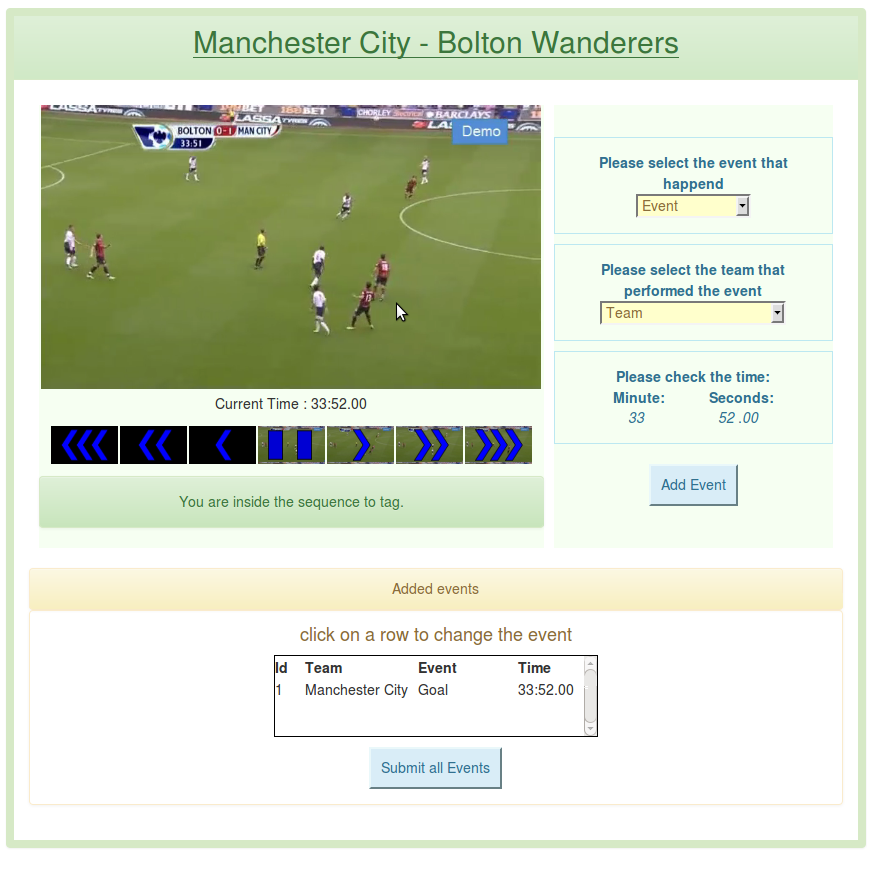
\includegraphics[height=5.5cm]{old.png}
			\end{figure}
	    \end{column}
    		\begin{column}{.5\linewidth}
    			\begin{figure}[p]
    				\centering
    				\caption{Neues Layout}
				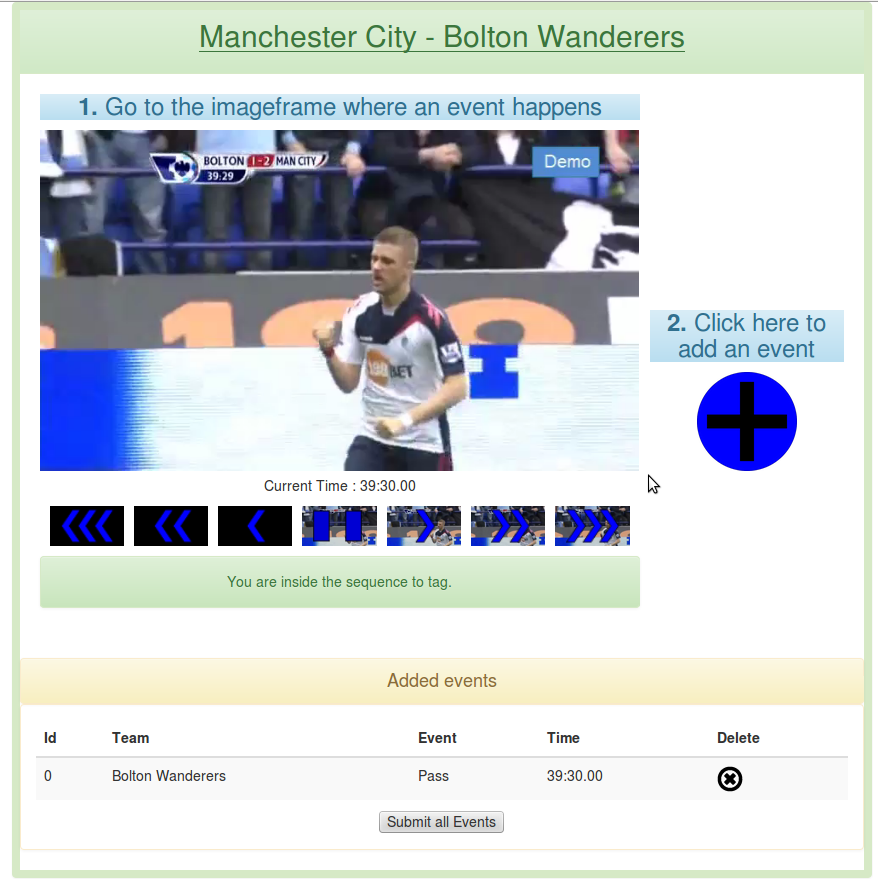
\includegraphics[height=5.5cm]{new.png}
			\end{figure}
    		\end{column}
	\end{columns}
\end{frame}

\begin{frame}
	\frametitle{Datenbank}
		\begin{figure}
    			\centering
			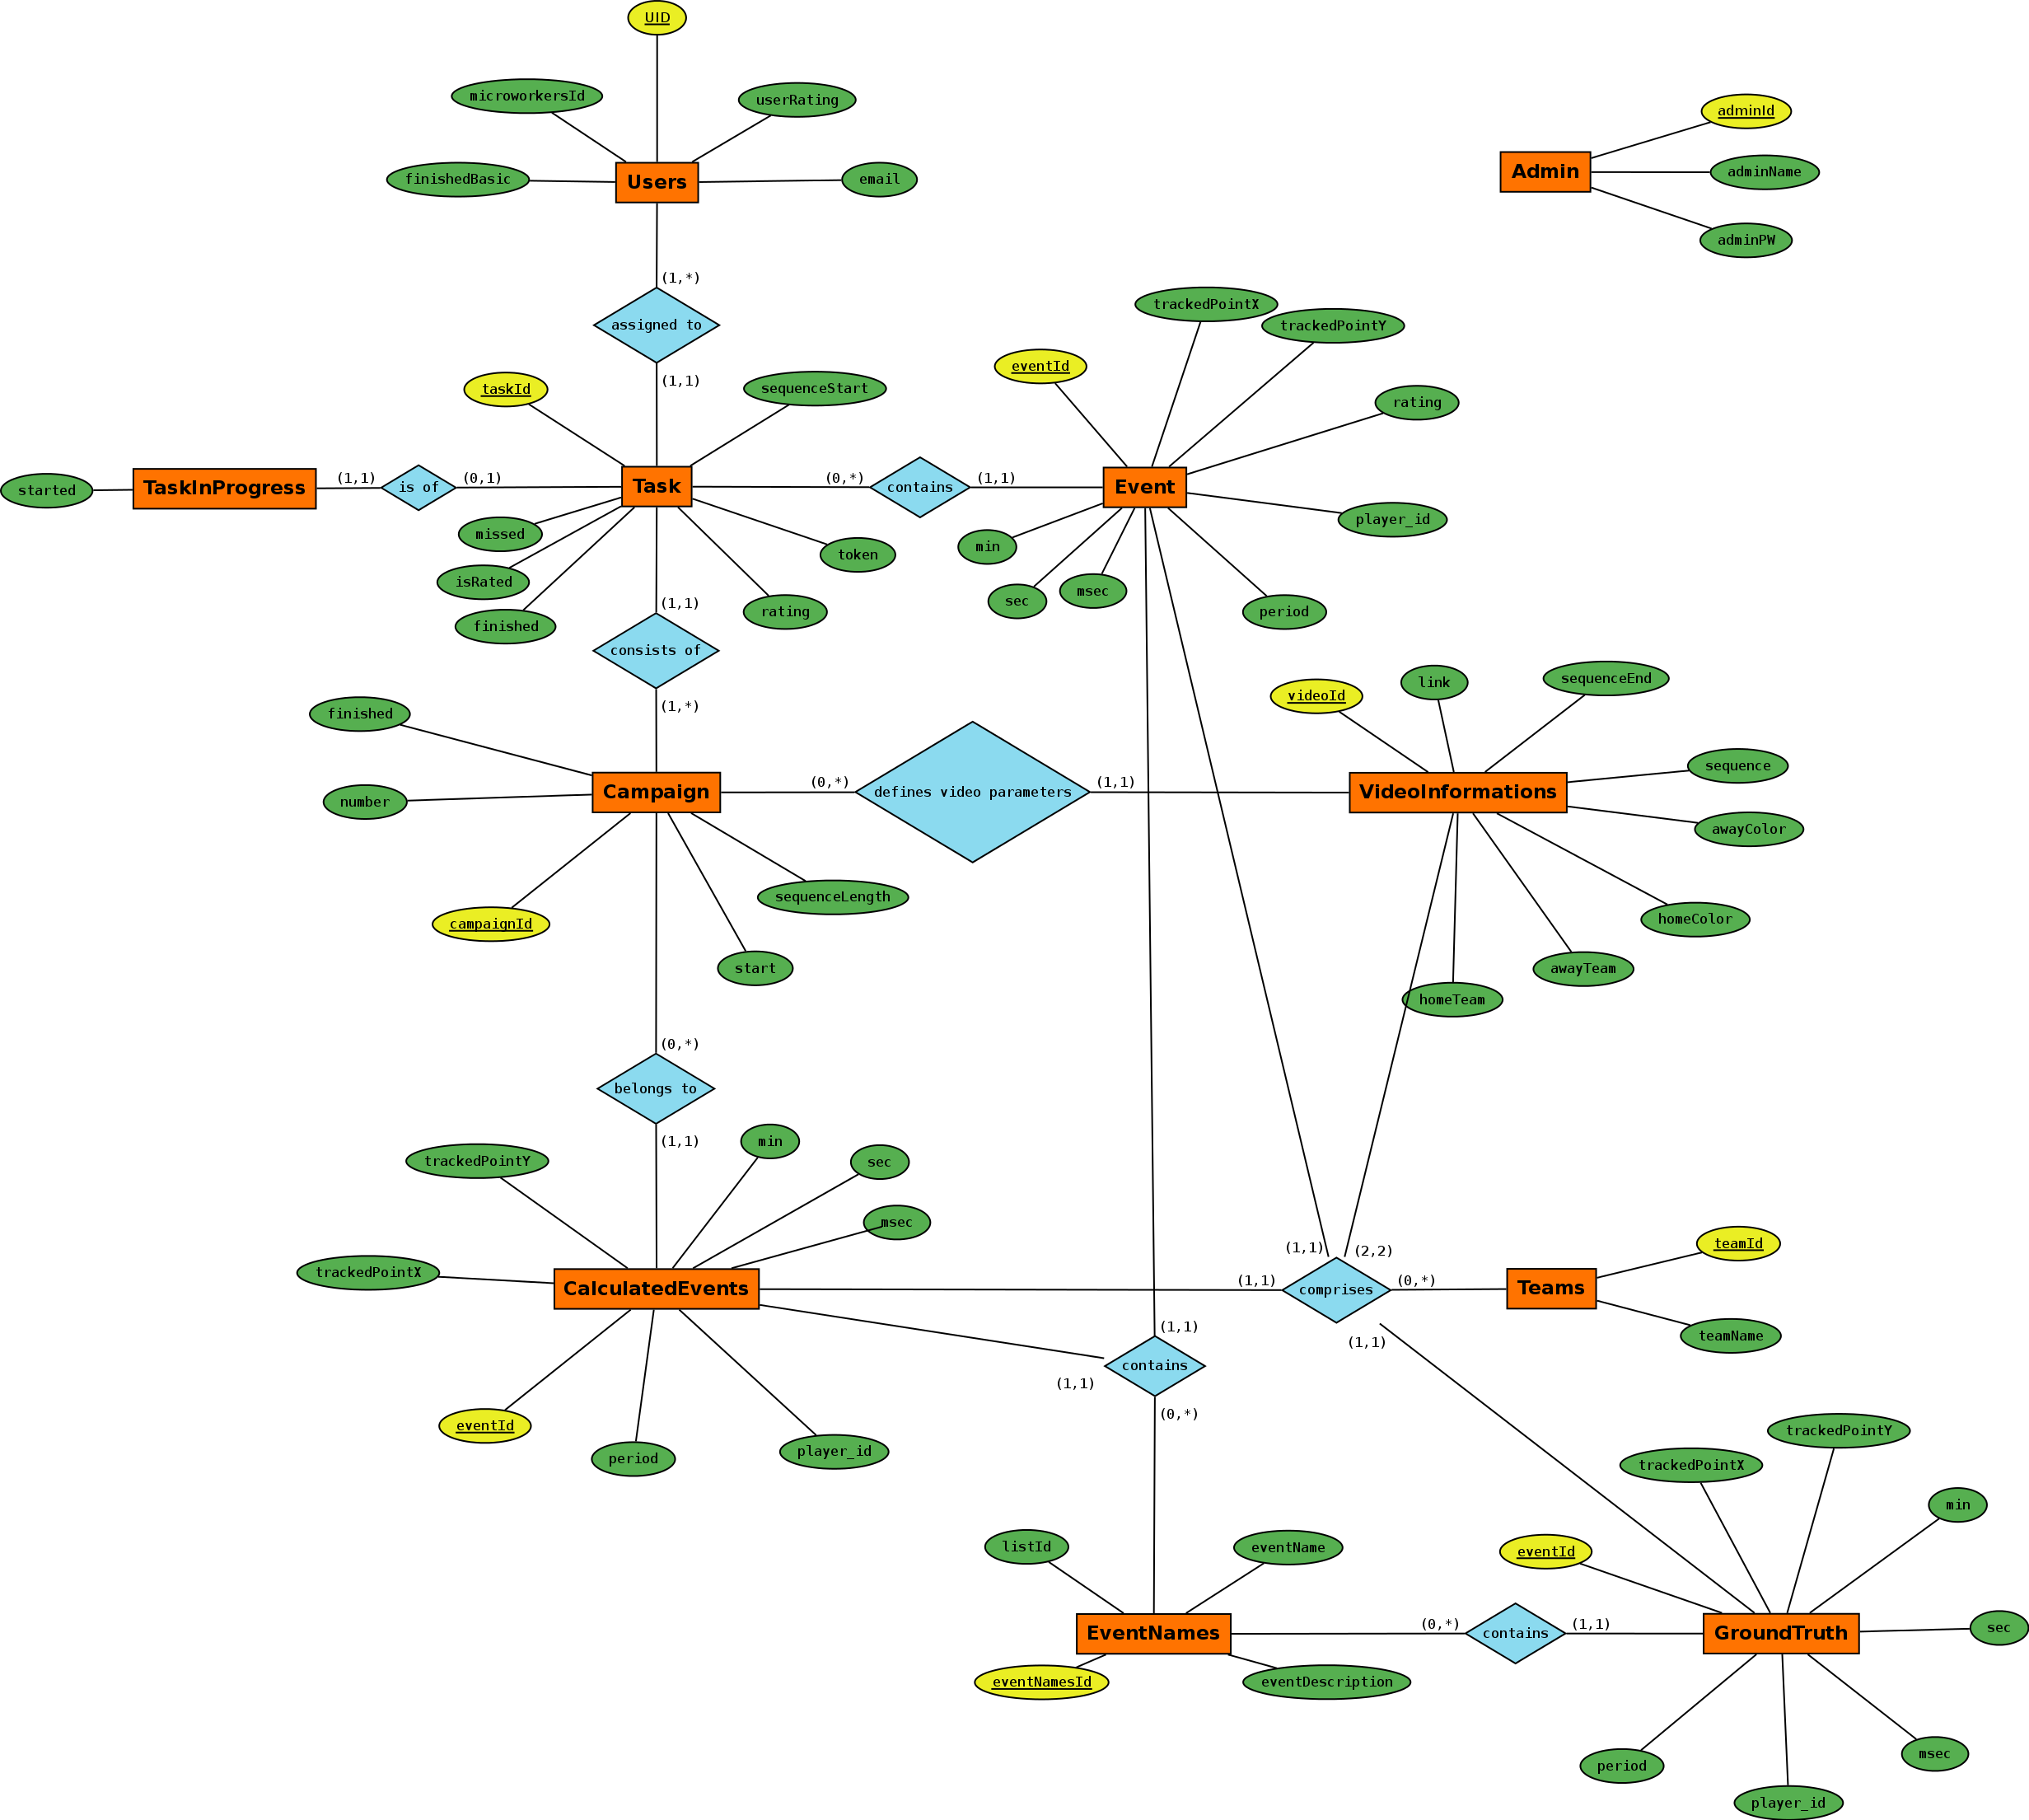
\includegraphics[scale=0.3]{ER_Diagramm.png}
		\end{figure}
\end{frame}

\begin{frame}
	\frametitle{Erster Test}
	\begin{itemize}
		\item Altes Layout
		\item 55 User, effektiv 53 User
		\item ca. 15 Stunden
		\item 82 beendete und 75 nicht beendete Tasks
	\end{itemize}
\end{frame}

\begin{frame}
	\frametitle{Auswertung der Daten}
	\begin{itemize}
		\item 23 schlecht, 53 in Ordnung
		\item Schlechte Daten:
		\begin{itemize}
			\item einige ohne Events
			\item mehrere Events zum gleichen Zeitpunkt
			\item komplett falsche Events (häufig Goals)
			\item Zeit häufig sehr ungenau
			\item Viele Tasks angefangen ohne zu beenden
			\item Mehr Tasks beendet als auf Microworkers
		\end{itemize}
	\end{itemize}
\end{frame}

\begin{frame}
	\frametitle{automatische Bewertung}
	\begin{itemize}
		\item Bisher von Hand verglichen
		\item zuerst jeden User gegen Basis testen, danach mit der jeweiligen Bewertung wahren Punkt finden.
		\item automatische Bewertung
		\begin{itemize}
			\item Rating Event: C$_{T}$ + C$_{Z}$ + C$_{P}$ + C$_{E}$ = C, C $\in$ {-1,1}
			\begin{itemize}
				\item C$_{T}$:= Kosten Team
				\item C$_{Z}$:= Kosten Zeit
				\item C$_{P}$:= Kosten Position
				\item C$_{E}$:= Kosten Event
			\end{itemize}
			\item UserRating = $\sum$ TaskRating = $ \frac{1}{N} \sum\limits_{n=0}^N$ EventRating
			\item verpasster Event oder -0.5
			\item UserRating zu Begin = 0, $\le$ -1 Warnung, $\le$ -2 keine weiteren Tasks
		\end{itemize}
	\end{itemize}
\end{frame}

\begin{frame}
	\frametitle{Probleme}
	\begin{itemize}
		\item Microworkers
		\begin{itemize}
			\item Task Pro Campaign und Benutzer nur ein mal
			\item Rating durch bestehende Benutzergewichte nur schwer umsetzbar
			\item Keine Kenntnis darüber weshalb in Datenbank 82 beendete und in Microworkers nur 53
			\item Task akzeptieren oder verwerfen von Hand
			\item Beta Version nur virtuell
			\item schlecht geratete Tasks werden neu zur verfügung gestellt
		\end{itemize}
		\item Video mit Slowmotions und Wiederholungen
	\end{itemize}
\end{frame}

\begin{frame}
	\frametitle{Nächste Schritte}
	\begin{itemize}
		\item neues Layout fertigstellen und testen
		\item automatisches Rating gegen Basis erstellen
		\item Tutorial Video erstellen
		\item erste Resultate niederschreiben
	\end{itemize}
\end{frame}

\begin{frame}
	\frametitle{Demo}
	Link zur neuen Version:
	\newline
\url{http://sportsense.cloudapp.net/WebProject/guided/Index.php}
\newline
\newline
	Link zur alten Version:	
	\newline
\url{http://sportsense.cloudapp.net/WebProject/without_login/Index.php}
\end{frame}

\end{document}

